
% Introduce the different experiments
% If experiment refer to each other, possibly also mention that here.

\chapter{Results \& Discussion}
The experiments performed during the project have led to many interesting results. Every experiment performed have had great impact on the AIs final performance (g: EVALUERING/ANALYS?). Either by presenting the problems and complications that the AI faces during learning or by providing a way to evaluate whether or not the modelling of the environment is sufficient.

This chapter presents and discusses the results that have been achieved during the project. The chapter is divided into sections by experiments performed. Each section presents results as well discussion and reflections about the experiments. The sections also introduce how different experiments and their results relate to each other. The order in which these results are presented follows the order in which conclusions were drawn and the project progressed (g: FOKUSERA PÅ LÄSAREN, INTE PÅ VÅRT PROJECT, TROR JAG). Thus one should get a general understanding of the AIs performance improvements during the project from this chapter.

% ----------------------------------------------------------------------------------------
% Refer to the description in method
% Present the results of the experiment
    % - What did it do?
    % - Fitness
    % - Generations required before results
    % - (Population)
% Analyse the results and the meanings behind them.
    % - Was it a good result? Why/Why not?
    % - What conclusions can be drawn from the results?
    % - How could we modify this experiment in order to get additional meaningful results?
% ----------------------------------------------------------------------------------------

% refer to the description in Method
% example: did it help to help in any way
% example: present data
% example: did the hypothesis work
\section{Fixed speed}
% constant speed -> focus on steering, one variable
% gradually increasing speed, method?
% increasing speed -> push the limits 

KEY FINDINGS: INTERPRET DATA WELL, FIND COMPLEX BEHAVIOUR, NOT OBSERVED TO OPTIMISE EVERYTHING IN THE SAME SOLUTION(?), HARD TO SEPARATE SIMILAR SCENARIOS, ...

By locking the speed of the car to a constant value, conclusions about the AIs ability to steer the car could be drawn. The constant speed was gradually increased with the goal to force the AI to modify the race line such that it takes wider corners, making it possible for the car to go around the track in such an efficient way as possible, given the current speed.

Noteworthy is that after the car completes a track, rewarding it for improved time or improved distance driven is analogous. Since the car is driving at a constant speed, this will only result in a shorter distance being driven to get around the track.

The experiment was performed in two ways, one where the AI can look further down the track and one where it only has local knowledge about the track. Results for each of these sub-experiments are presented in the subsections below.

% By locking the speed of the car to a constant value, this experiment aimed to evaluate the networks ability to steer the car. The speed was initially set to a value that was known to be low enough for the car to be able to take a lap by driving in the middle of the track at all times. The speed was increased gradually, trying to force the AI to take wider race line in order to get around the track with the higher speed.

% After it completes a track, rewarding it for improved time or improved distance driven is analogous, since it drive at a constant speed.

% NOTE: I am not certain that some results are actually correct in this section. Does it actually stick to the middle? I do not believe that I had that behaviour when I ran the experiment on the cloud computer. Can't visualise it atm though.
\subsection{Only local perception}
When the AI is not provided with any information about how the track looks in front of the car, the car sticks to the middle of the track. Since the AI only has knowledge about the track in a small space around the car, it never adjusts for corners before they are actually next to the car. This means that when the car eventually encounters a corner, it will appear as though the car is no longer in the middle of the track. At this point the AI tries to recover the car and position it in the middle of the track again. This lead to late reactions, making it impossible to get past tight curves if the speed was too high simply by reacting to the distance from the middle as the curve appears.

The AI tries to compensate for these late reactions by increasing the amount of steering applied. This causes the car to oscillate around the tracks mid line. The oscillation occasionally helps the car to position itself correctly before a tough curve. Which further helps the car to complete the corner. The oscillation only occurs after the first curvature on the track, since that is the point in which it has to start compensating. Eventually the AI learned to minimise the oscillation and the car seems to simply stick to the middle of the track.

When the cars speed was pushed to values that requires the car to take wider curves then sticking to the middle, the car failed to make a complete lap. The amount of steering required in order to complete certain curves from the middle of the track is simply larger than the available turning radius, and the oscillation required to compensate for this forces the car to drive outside of the track or failing other corners.

The speed was initially set to 10 m/s, which resulted in the car managing to take a lap on generation 2. The speed was then gradually increased to 11.6, 11.7, 11.75 and 15 m/s. At 11.6m/s the car managed to make a complete lap after 5 generations. At 11.7 m/s, the car managed to make a complete lap at generation 22. Further increasing the speed resulted in the car not taking a complete lap.

% Storlek och vilka indata som används.
%[Network structure...]

% TODO: Add some more reflections
The only way it can know there is a curve, is if it find itself away from the middle. It is therefore impossible for it to sophistically prepare for an approaching curve. The only way it improved after a certain degree was if it found an accidental oscillation, where it started to steer before the start of a curve. It is an unstable solution which did not work for several subsequent difficult curves.

[Does it behave differently with edge distance data instead or in addition to distance to middle data? Will it stick to another lateral position than the middle?]

% OLD TEXT:

% When the constant speed was increased, the car started to oscillate around the mid line of the track. The oscillation however only occurred after the first curve in the track, which was interesting. The oscillation sometimes helped the car to position itself in a better way for a tough curve, which in turn helped it to complete that curve. Oscillation will however cause the car to drive a longer distance, compared to driving in a straight line. After completing the track, if the oscillation was not needed for taking a specific curve, it always stopped. The network managed to learn to make it stable. 

% The car stick to the middle of the track. If it drives in to a curve and appear away from the middle, it tries to recover. If it approached a tight curve, it would not perceive the curve until it suddenly appear to drive away from the middle. This lead to late reactions, making it impossible to get past curves if they were to tight or the speed was too high.

% It usually resulted in oscillations around the mid line, usually after some disturbance like the initial curved. Some times the oscillation made it get in better position for a difficult curve, allowing it to complete the curve better. 

% Oscillation will cause the car to drive longer than if it would drive straight. After completing the track, if the oscillation was not needed for taking a specific curve, it always stopped. The network managed to learn to make it stable. 

% The only way it can know there is a curve, is if it find itself away from the middle. It is therefore impossible for it to sophistically prepare for an approaching curve. The only way it improved after a certain degree was if it found an accidental oscillation, an unstable solution which did not work for several subsequent difficult curves.

% Training times...

% Network structure... 

% [Does it behave differently with edge distance data instead or in addition to distance to middle data? Will it stick to another lateral position than the middle?]


\subsection{Local perception and track curvature}

% Ser vi något intressant om vi ökar hastigheten
% Beteende:
% - Klarar högre hastigheter
% - Svänger före kurvorna
% - Tar mer höjd inför kurvorna
% - 

% Beteendeanalys:
% - tolkar datan bra
% - beter sig i stora delar som man kan förvänta sig
% - Begränsad av hastigheten och bilens prestanda, som vi ser när man ökar hastigheten att beteendet blir "sämre"

% Data:
% - när tar den ett varv
% - när blir det optimalt
% - storlek på nätverket och vilka indata

% Analys:
% - Vilken data användes för det här problemet/beteendet?
% - Hur lyckades NEAT hitta något
% - Kan den lära sig flera saker samtidigt?

It is interesting to investigate how much the AI can manage to improve if it has access to the curvature of the track ahead. 

We found solutions that managed to complete the track with speeds up to 12.1 m/s, compared to 11.7 m/s without the track curvature data. The difference in speed may seem small, but the difference in behaviour is substantial.

What these solutions generally do is that they position themselves well before a curve, to compensate for the larger turning radius. They also start to steer before the curve actually start.

The speed that provided the most correctly looking race lines was 12.0 m/s. At that speed the AI had to push the limits in order to manage the toughest chicane. When the speed increased, the AI had to start turning very late in the chicane, to make a little more space for the following curve. This made it less interesting to investigate further, since that behaviour resembled real behaviour less.

% Check for longer training sessions
Each of the solutions found showed some typical characteristics. If one solution managed to drive tightly to the inner side in the toughest curve or positioned itself extremely before a curve, it also showed that tendency for all other mayor curves. On the contrary, if it turned late in the tough curves, it also did it for the other curves too.

%Check for longer training sessions
The recurrent characteristics in the behaviour for a particular solution often had one limitation, that they failed to manage simpler as efficient as the tough curves. If the solution managed to take the tough curve, near optimally, we never observed that it also managed to take the simpler curves as efficiently. For example, for the lightly turning curves, the car always drove a few meters from the edge of the track, even if it certainly had traction to stay closer. 

%Check for longer training sessions
It seemed like it did not learn to distinguish properly between the different difficulties, and simple did the same behaviour in miniature. Worth noting was that these training sessions lasted for only about 2-600 generations. We have not proven that it is not possible if one trains for longer.

The best network found for the speed 50.0 had fitness 5821.93. It had a total of 9 hidden nodes, a total of 20 edges, 8 edges within the hidden layer, 4 to output nodes, 9 of the input nodes and bias was connected (0, 1, 3, 4, 5, 7, 8, 10, 13, 15) (bias, distance to middle, distance to right edge, angle to mid line, curve data points 10m 42m 66m 144m 397m and the segment sum of the first four points in the region 10-66m) (Remember to check which edges are enabled!)


\subsection{Shortest path}

The fastest route for a car that moves forward with a constant speed is the shortest one. This means that the only way for a genome to increase its fitness once it completes the circuit is to decrease the distance driven around the track.  

The result show that after the algorithm finds specimens that are able to complete the circuit, the gene pool continues to improve. The path around the circuit is shortened to a great extent. The difference in length of the raceline and the midline of the circuit is significant. 

The optimal behaviour is intuitively to always drive on the inner curves and to drive a straight line between the curves where it has to turn. Small variations on the curvature should not matter, if the edge does not intersect with the path the car drives.

The car follow the key behaviour aspects, but not to the extent that the path is optimal. We can see that it drives tightly to the inner side for very tight curves, but not for low intensity curves.

Training times...

Network structure...


%\section{(Existing steering controller)}
% refer to the description in Method
% example: did it help to help in any way
% example: present data
% example: did the hypothesis work

\section{Steer and speed control}
KEY FINDINGS: SIGNIFICANT INCREASE IN COMPUTATIONAL COMPLEXITY, FEWER OPTIMAL ASPECTS(?), ...

% refer to the description in Method
% example: did it help to help in any way
% example: present data
% example: did the hypothesis work

% Beteendeanalys
% - it do optimise for time!
% training, data,

% Analysis
% - Similar times as for the fixed speed
% - How do the behaviour/ performance differ to the fixed speed. 
% - Longer training time => more complex
% - Can it manage to learn many components of the behaviour at the same time? One component only may make the performance worse
%

When the AI is given steering and breaking as a second output, the complexity of the computations increase significantly according to the results. It takes this experiment 506 generations until a genome can complete a single lap around the track. Even though this genome would have the ability to both use the break and throttle, it would still hold a lower average speed than the best genomes would in the constant speed with track curvature in the previous experiment (Shorten sentence).

When a genome manages to complete a lap around the track, the AI actually tries to minimise the time it takes to complete a lap. 


\begin{figure}[h]
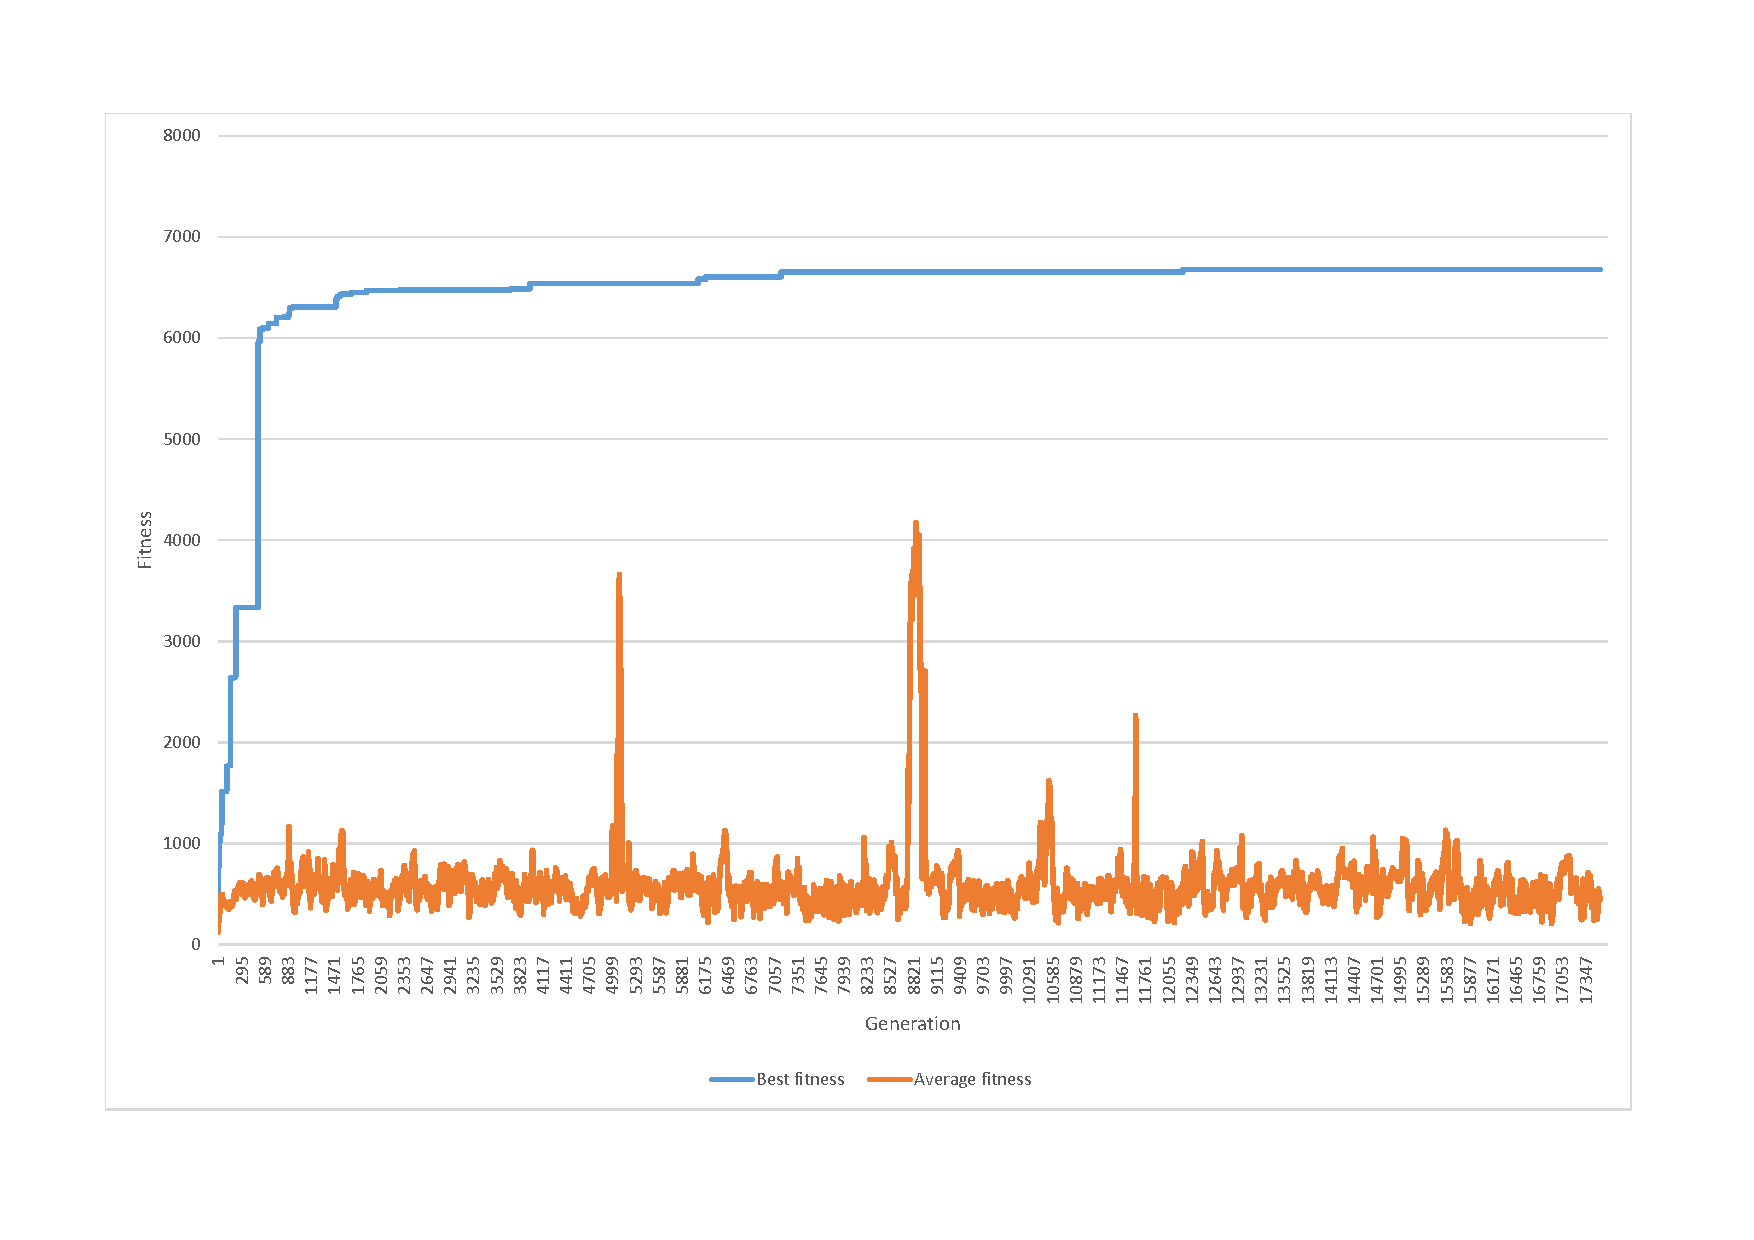
\includegraphics[width=16cm]{report/images/graphs/fitness}
\centering
\caption{Showing best fitness and average fitness of each generation}
\end{figure}

As can be seen in the graph above (insert proper tagging), the car AI creates a genome that reaches a fitness higher than the termination distance at 5200 in relatively few generations. Once this fitness level of 5200 is reached, the algorithm tries to optimise the time spent driving. The p

\section{Single short track segment}

% \section{Multiple short track segments}

\section{Mirror track}
%Train at one track, then drive it on the mirrored track


%- If it is trained for certain tracks, can it manage others?



\chapter{Discussion}


\section{The neat mechanism}
%   - Neat train to fulfil a declared goal, it is not a description on how to do it
%     - The fitness value say how good a genome is
%     - It do not base its decisions upon previous path of progress
% X - Analysis: How entangled is a neural network? Can one part evolve safely without disrupting other parts? Is it possible to evolve safely? Catastrophic forgetting?
% X - Ability to manage multiple goals? Can it achieve one or several tasks at the same time?
%   - How well do the greedy approach work?

%   - What are the properties for getting stuck or to develop innovation? 
%   - Do it exist certain statistical improbabilities or unavoidableness?
%   - How will the stochastic parameters in neat influence the performance? 
%   - We see that many early solutions have very few nodes, solutions that have gone through long training have many. How much do the performance really differ? 
%   - Often only few of the input values are covered.

%   Wild ideas/suggestion:
%   - An image Daniel presented, showed during a long training, it was rare that networks made it around the track. After it succeeded to improve the results, or get around the track, the performance was always lost shortly after (?). Does this show that the neat algorithm in the setup we used it, is not efficient? Is avoiding local minima, too aggressive?
%   - In the neat paper, the authors stated that the training often got stuck for a while. Then, when some kind of archetype structure was found, the performance could then quickly increase as good networks was derived from the archetypes. It is not far fetched that the two steps in the process have different requirements. Maybe archetype topologies are smaller and faster to sieve. The elaboration of an archetype maybe requires more processing, as it might involve larger structures and thus larger need for tuning and compensation when evolving. Suggestion: Change the stagnation limit (and possibly other parameters) as the number of generations increases, or when certain properties relating to the role a species/genome hold. It might not be possible to find a sweet spot that works for all situations. 
%   - What has progressed after a leading genome has stagnated and died?
%   - What size of a network is beneficial for a network to probably to be an archetype? small? connect to all input values, or cover all categories of inputs? After a successful 
%   - How general will this approach be? If it is successful, will it only be it for problems that resemble characteristics from the racing problems? If, so what aspects? If not, what characteristics do it solve/target?

As previously described, NEAT is detached from the the actual problem it solves. It do not do any particular analysis of the problem and very little analysis of the results it collects along the way. The feedback it get from the problem is the fitness value. One might question how much information that single value can provide in the process of solving complex problems.

NEAT progressively builds up networks. Even if many different networks are evolving concurrently, each of them evolves in small steps. The number of changes for a particular network are rather limited for a single generation.

This requirement for a species to succeed is that the mutations for the individuals that are rewarded most, also are mutations that lead to the end goal. If they are not locally rewarded enough, they will be discarded and if the whole species perform too poorly it will go extinct for the benefit of other species and individuals that may or may not reach the end goal.

Information are hidden from the neat algorithm, it do not know or understand what it do good or what it fails with, so no directed modifications can be applied. It depend on that a better solution is withing reach of one of the currently genomes active in the pool.

% TODO DISCUSS ANALYSE
%HOW much can it try before extinction?
%stagnation. specie comparison. knoppa av sig, liknande återkommande.
If a network perform bad in comparison to the others in the same specie, or if a specie perform too bad in comparison to the other species they will be discarded.


% HOW much can a solution change, how well tuned do it have to be in order to work? To some extent, it have to make sure that the previous definition space / manageble scenario space is not tempered with, as it expands definition space. How entangled is a network? 

% Det finns en mekanism för att klara av stillastënde, men temporära nedgångar är riskfyllda. Därför vill man att det ska finnas en jämn utveckling serie för att ta sig vidare. Det kan hjälpa att fitness efterspeglar utvecklingen. Låser man in beteende genom att fokusera på vissa resultat, borde man fokusera på att hitta. Utforma träningen så att den inte får för stora steg i fitness. snabbt krascha i sista svängen eller ta sig runt. Konsekvenserna borde inte vara så stora av att misslyckas så man inte vill lära sig något nytt.
% Borde man fokusera på att mäta beteendefaktorer istället för resultat? Ett logiskt steg närmare.
% Köra långsamt hela banan eller bra halva



%WHAT happens when the leading species die? HOW much progress are handed over to other species?



% CAN it improve on multiple goals, or only once at a time? How do it manage to learn behaviour with in-exclusable components?
% It is possible to add multiple edges in a few number of generations, but it is unlikely that they are the relevant ones and that they are well tuned. e.g. gas and brake. Kanske ofta utveckla en sak i taget.
% Motsträviga mål, tex ändra sväng för att hantera annan hastighet. Svårt att göra om en sak måste göras i taget. 




% TODO, CONNECT TO THE RESULTS WE HAVE OBSERVED
RESULTS. We can see in e.g. shortest path that it finds beneficial behaviours, that often resemble the same characteristics. But it seldom learn all of the smaller details. We have not observed that it solves everything, and are together with the discussion above suspicious on wither it is able to succeed with it to.

Although the discussion deducted from the key mechanics of NEAT and the results from our study do not prove that NEAT cannot find a complete and all-round optimal solution for the kind of problem we investigated, it highlight a structural weakness.



\section{Problem modelling}
- Information and/vs simplicity. 

- We want to provide the necessary amount of information, as compact as possible. For example, it would probably be much more difficult for it to interpret the vector points in the representation that the simulator uses. The curvature data is much more compact

- Simplicity of the format of data is highly beneficial if not crucial (simplicity in the sense that it is close the format it can be used in). Processing of data might probably increase the complexity of the training several magnitudes, as it both would require processing and interpretation.

- However, if data is pre processed to extract some kind of property of the data other information might be lost. In order to not loose necessary information a greater number of inputs might be required, which may in itself increase the complexity. Example: Curve data points as today, but with values on how sharp the curve inside the segment is, then two floats are needed instead of one and one might think it is better to simply double the resolution of points instead.

- In context of neat and curvature data: Fixed position is a compact representation. Information lay in the index/topology. In order to interpret distance to an observed object a structure in topology is required. If the exact distance for which some action should need to change, the topology need to change, which is a difficult task. Index based distances for actions maybe require an abstraction layer on top of the input in order to make them parametrised. Could an interpreted object input model improve the adjustment capabilities, example touple with distance to the curve and its properties? Then some more of the interpretation lie in the weights and not in the topology itself. modifying the topology is expensive and probably in most cases statistically impossible.


\section{Neat usability}
% - How well do it perform with not knowing how things work?
% - For how large and complex problems can it perform?
% - In our experiments it controlled the car at a low level, can improvements be made if it is modelled differently by the programmer? Added abstractions? More supplemented by other parts of a solution? Several single purpose networks in modules?
% - How much domain knowledge is required to make it ok/very good?
%   - Degree of knowledge?
%   - Type of knowledge? Examples: Structural knowledge provided by the programmer, example data, experience
%   - Worth noting: excluding something unimportant also prove a kind of knowledge
%   - Might be good in a situation where one know what behaviour is wanted, but not how to accomplish it.
% - Find a fitness function that gives smooth progress to the maximum, with as few local maximums as possible. 

As previously described, NEAT is not an algorithm designed to solve a particular problem. Instead it produces artificial neural networks through neuroevolution with reinforcement learning. The process is solely controlled by the fitness value.

This abstraction of the actual problem has two sides. Firstly, the simplicity make the usage easily implementable as few domain specific processes are needed. In case it manages to solve the problem sufficiently it require little domain knowledge from the developer, as the algorithm managed to solve the problem on its own. On the other hand, if the result is not sufficient, the solution is not easily modified. Improvement probably require action on a system level, either the actual training or the application of the neural network(?).

...

\section{Comparison to other algorithms and concepts}
- How do it stand to other algorithms?

- Compare degree and type of domain knowledge needed? Example of types: Structural knowledge provided by the programmer, example data, experience



%Generality of results
%- How stable and general is it? Can it manage the same curve in different situations? Stability for unpredicted factors?
%- Over training. What do it mean, is it a risk and can it be avoided?

% Dicuss generality of the discovered behaviours
% Relate to the experiments, especially mirror track. 
\section{Generality of results}
One goal of the project was to find general behaviours, which means that the system should learn to drive on many different circuits instead of memorising a script of how to drive on a specific track. We showed in the mirrored track experiment that ..!!!!.. . Though that is not the only aspect that affect the generality of the solution. 
There is also the possibility of over-fitting the neural networks to the specifics of the training environment. This means that a behaviour is found that by chance works well on the training circuit, but not in general. For example if the system learns to distinguish specific locations on the track and take decisions based on which segment the car is located in instead of the track shape.


\section{Conclusion}
- Summarised evaluation of neat and other concepts dealt with in the report

- What do it mean for ML in general?


% Discussion of the behaviour
% Present current results
% This chapter presents and discusses the results that have been achieved during the course of the project. We successfully present the car driving around the track. However the lap that is taken by the car is neither optimal in respect to the race lines nor the time that it takes for the car to travel around the track.

% The experiments performed during the course of the project have given varying results. Every experiment have had a large impact on how the project has progressed and on the final results. The results for each experiment and the conclusions that could be drawn are presented and discussed in this chapter.

% \section{Experiments}
% Introduce this section somehow.

% \subsection{Curve Data as input}
% Present and discuss what results this method achieved for us.
% What kind of machine learning techniques did we use? What did they do differently?
% What behaviour did we see? Why is that?
% Is this behaviour similar or identical to a real race-car driver?
% Is it the most optimal route around the track, with regards to lap time?
% Can we expand this solution further? If so, how?

% This experiment was the first one that was carried out with any real progress towards the goal. We managed to produce a machine learning algorithm efficient enough to drive the car around the track without crashing, however given some simplifications; The car automatically accelerates in a straight line, up to a certain point where it stops accelerating and keeps the same constant speed. The neural network has the possibility of controlling the amount of breaking and turning the car does, overriding any automatic acceleration that the car does by itself.

% This results in a neural network successfully driving the car around the track. However the path taken is not the optimal one. The path starts of by oscillating left and right between the middle of the track. After a few generations of training, the neural network starts to adjust the oscillating such that the sharper curves can be taken with a wider radius. Given even more training the oscillating almost disappears completely, it only remains before and after some curves.

% This behaviour is as mentioned of course not optimal, and neither is it one that a human race-car driver would chose to take. It is both longer and more complicated than would be required for simply driving around the track, without optimising for maximal speed or time.

% The training algorithm seems to converge towards a simple neural network between all of the training sessions that has been performed. The neural network produced is one with only one connection between an input and an output. The training required in order to make a complete lap, takes no more than a few minutes. These factors leads us to believe that we can increase the complexity quite significantly before the search space has become to large to be solved within a reasonable time. Thus the limit of NEAT with respect to our problem has not been reached yet.